\chapter*{Introduction}

Le differenze tra computer vision, robot vision e elaborazioni delle immagini 
sono molto sottili:
\begin{itemize}
    \item \textbf{computer vision}: si usano le immagini per comprendere la scena 
    invertendo le proiezioni. In sostanza si parte dall'immagine per ottenere la 
    scena geometrica
    \item \textbf{robot vision}: molto simile a computer vision con la differenza 
    che si utilizzano ulteriori sensori come LIDAR ecc\dots
    \item \textbf{elaborazioni delle immagini}: si occupa di estrarre delle feature 
    dalle immagini date
\end{itemize}

\section{Modelli Pin-Hole}
Le immagini sono la base della computer vision e il modello più semplice di 
proiezione dell'immagine tridimensionale sull'immagine due dimensioni è il pin-hole.

Questo è uno dei primi modelli, nella figura \ref{fig:pin_hole}.
\begin{figure}
    \centering
    \includegraphics*[]{./figure/pin-hole.png}
    \caption{Esempio del modello pin-hole}
    \label{fig:pin_hole}
\end{figure}

Il modello si basa sull'avere una bariera tra il piano due dimensioni e l'oggetto
inquadrato, sul quale è presente un piccolissimo buco, chiamato \textbf{pin-hole},
talmente piccolo da far passare un solo raggio di energia riflessa dall'oggetto e
farlo cadere sul piano di proiezione. Questo modello è una \textbf{proiezione prospettica}
quindi oggetti vicini sono più grandi di oggetti lontani e le rette parallele risultano 
incidenti in un \textbf{punto di fuga}.

A livello puramente geometrico, si ha un piano $uv$ bidimensionale di proiezione (piano immagine)
con centro in $o_i$, si ha poi il centro dello spazio tridimensionale $xyz$ composto dal 
punto $c$ centrato nel pin-hole. L'asse $z$ sarà detto \textbf{asse ottico}, la 
distanza dal punto $c$ e il punto $o_i$ è detta \textbf{distanza focale} ed è segnata 
come $f$. La formula matematica che descrive questo modello è un sistema di proporzioni:

$$P:Z = P':f \equiv \left\{\begin{array}{c}
    \frac{x}{z} = \frac{u}{f}\\  
    \frac{y}{z} = \frac{v}{f}\\  
\end{array}\right.$$

\begin{figure}
    \centering
    \includegraphics*[scale=0.2]{./figure/pin-hole-modello.jpg}
    \caption{Modello matematico pin-hole}
    \label{fig:pin_hole_model}
\end{figure}

Dove $x,y,z$ sono le coordinate del punto nel mondo, $u,v$ sono le coordinate 
della proiezione e, infine, $f$ è la distanza focale. La formula ha tre diversi 
scopi:
\begin{itemize}
    \item quando fissiamo $x,y,z, f$ abbiamo la proiezione del punto $P$ del mondo 
    sul piano $uv$
    \item quando abbiamo $f,u,v$ allora otteniamo la retta di interpretazione del 
    punto $p'$
    \item quando conosco $u,v,x,y,z$ effettuamo la calibrazione del modello e otteniamo 
    la distanza focale che ci permette di ottenere quella proiezione
\end{itemize}

Ricorda che quando abbiamo un punto e vogliamo trovare la sua posizione nel mondo
non possiamo ricavare il punto originario della proiezione ma abbiamo solo una retta 
di interpretazione del punto. Questo è dovuto dal fatto che si ottene una retta, 
si può ricavare la distanza originaria usando stereoscopia o sfruttando le informazioni
globali dell'immagine.

Il limite fisico del modello è la dimensione del buco che è impossibile sia 
così piccolo. In aggiunta se fosse così piccolo allora si avrebbe un'immagine molto 
buia, per risolvere questo problema dobbiamo far entrare più luce e questo implica 
il fatto che passano più raggi per ciascun punto che si sovrappongono con i raggi di altri 
punti (\ref{fig:hole}).

\begin{figure}
    \centering
    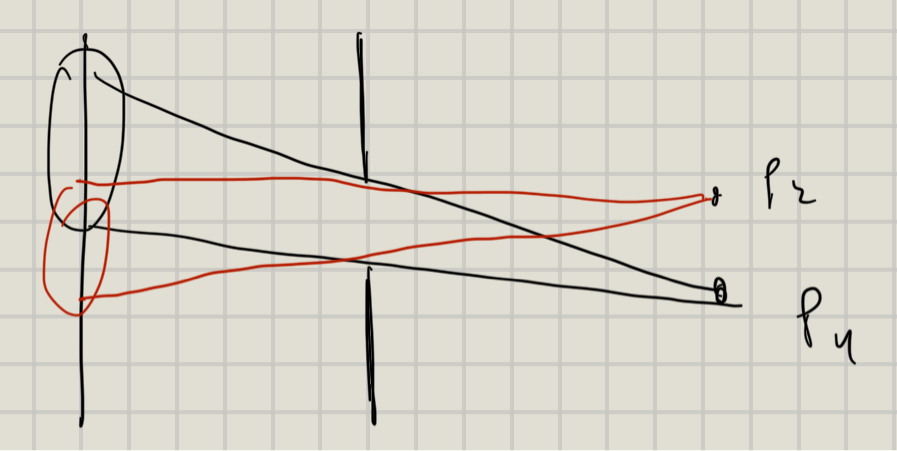
\includegraphics[width=0.5\textwidth]{figure/example_hole.jpg}
    \caption{Esempio di ingrandimento del buco}
    \label{fig:hole}
\end{figure}

Per risolvere questo problema possiamo utilizzare delle lenti fotografiche che 
da un aumento di dimensione del buco concentrano i raggi in un unico punto.

\section{Modello di proiezione}
Prima di introdurre le lenti bisogna parlare delle varie proiezioni che si possono 
avere oltre a quella propsettica.

La prima è quella \textbf{ortografica} che è quella utilizzata dai teleobiettivi
delle macchine fotografiche, la proiezione ortografica trasforma tutti i raggi incidenti
sulla lente in raggi paralleli. Per questo si richiede un ristretto angolo focale(\ref{fig:ortography}).

\begin{figure}
    \centering
    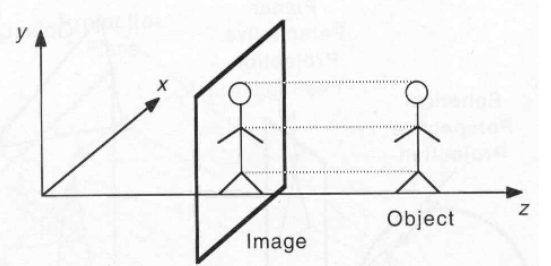
\includegraphics[width=0.5\textwidth]{figure/proiezione_ortografica.png}
    \caption{Esempio di proiezione ortografica}
    \label{fig:ortography}
\end{figure}

La prima è quella \textbf{ortografica scalata} che è quella utilizzata in ambito 
industriale. La proiezione ha una proiezione dei raggi in modo ortografico 
ad una certa distanza per distanze differenti si ha un effetto prospettico. Questo 
è usato nelle industrie per le telecamere che analizzano oggetti alla stessa distanza.
(\ref{fig:scalata_ortography})

\begin{figure}
    \centering
    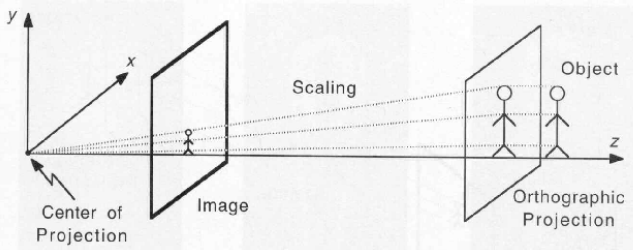
\includegraphics[width=0.5\textwidth]{figure/proiezione_ortografica_scalata.png}
    \caption{Esempio di proiezione ortografica scalata}
    \label{fig:scalata_ortography}
\end{figure}

\section{Lenti}
I dispositivi ottici si possono basare:
\begin{itemize}
    \item riflessione
    \item rifrazione
    \item entrambi
\end{itemize}

Definiremo la \textbf{distanza focale} della lente ovvero la distanza dalla lente 
alla quale si concetrano tutti i raggi paralleli che incidono sulla lente.

Le lenti funzionano seguendo lo schema in figura \ref{fig:physical_lenses}.

\begin{figure}
    \centering
    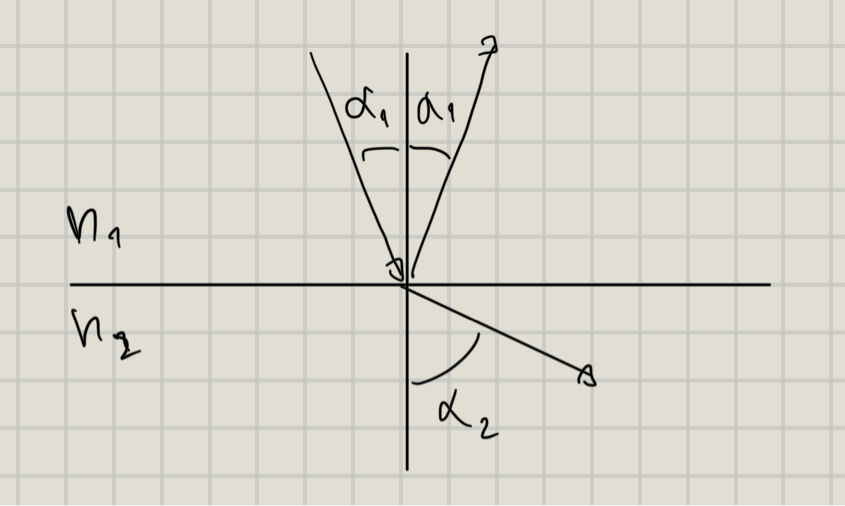
\includegraphics[width=0.5\textwidth]{figure/lenti_fisica.jpg}
    \caption{Schema fisico degli oggetti}
    \label{fig:physical_lenses}
\end{figure}

Dove $\alpha_1$ è l'ancolo di incidenza e riflessione della luce mentre $\alpha_2$
è l'angolo di rifrazione, al tempo stesso $n_1$ e $n_2$ sono i coefficienti di 
riflessione e rifrazione del materiale.

In generale verranno introdotti soltanto lenti basate sulla rifrazione e quindi 
vogliamo minimizzare la riflessione, quindi vogliamo evitare l'\textbf{angolo critico}
 che è l'angolo in cui la luce viene solo riflessa ma non rifratta.

Il modello della lente a livello fisico è dato dalla \textbf{legge delle lenti} 
basata sul modello \ref{fig:model_lenses}.

\begin{figure}
    \centering
    \includegraphics*[width=0.5\textwidth]{figure/legge_lente.jpg}
    \caption{Modello della lente}
    \label{fig:model_lenses}
\end{figure}

La legge è 
$$\frac{1}{f} = \frac{1}{z} + \frac{1}{Z}$$

Dove se $f$ è la distanza focale $z$ è la distanza della proiezione dall'altra parte 
della lente e $Z$ è la distanza dell'oggetto dalla lente. Da notare che $z$ e $Z$
sono discordi perché sono posizionati dal lato opposto rispetto alla lente.

Da notare che per regolare l'ampienza del buco si parla di regolazione del diaframma,
più è ampio il buco, maggiore è ampio il diaframma e più luce entra. Questo serve 
per regolare l'apertura del diaframma quando la luce è intesa o scarsa. Se è buio 
allora non si vedere nulla.

Per quanto riguarda l'effetto di focatura, un punto è a fuoco quando il diametro di
sfocatura è nullo. Il problema è che quando gli oggetti sono a distanza variabile 
allora dobbiamo trovare il modo di cambiare la sfocatura e questo si basa sullo 
spostare il piano immagine o la lente per raggiungere un diametro nullo. Il problema 
che solo i punti ad una sola distanza sono a fuoco tutti gli altri sono sfocati, 
per risolvere questo problema sfrutta la discretizzazione delle immagini usando i 
pixel. Ovvero quando vogliamo ottenere l'immagine andiamo a ottenere una matrice 
di pixel, questa matrice sarà discreta e si avrà uno spazio tra un pixel e l'altro.
Questo è utile per risolvere il problema della sfocatura infatti per vedere a fuoco 
un punto basta far sì che il diametro di sfocatura non occupi più pixel ma uno solo.
Per regolare il diametro basta agire sul diaframma e sul fuoco.

Regolando il diaframma possiamo avere anche profondità di campo diverse della scena
come si può vedere nell'immagine \ref{fig:prof_campo}.

\begin{figure}
    \centering
    \includegraphics*[]{./figure/profondita-campo.png}
    \caption{Esempio profondità di campo}
    \label{fig:prof_campo}
\end{figure}

Delle lenti abbiamo anche l'angolo di visione o \textbf{field of View} che è l'angolo 
di raggi che entrano nell'obiettivo rispetto all'asse ottico. Questo angolo forma 
un cono e successivamente si ha cerchio di riflessione sul sensore o sull'immagine, in generale
si cercherà di avere un cerchio di riflessione più grande rispetto al sensore.

Il FOV può portare a distorsioni dell'immagine per oggetti sul confine dell'occhio visivo:
\begin{itemize}
    \item aberrazioni cromatiche: strisce di colori dovute alla rifrazione ad angolature diverse dei colori
    \item distrorsioni: distorsioni delle proiezioni dei punti, questo è dovuto 
    dalla deviazione dei raggi della lente. Possiamo avere distorsioni radiali (barilotto o cuscinetto) o
    tangenziali (traslazione di punti)
\end{itemize}

